\chapter[Paper II:\@
  platinum-triggered bond-cleavage of pentynoyl amide
  and \emph{n}-propargyl handles for drug-activation]{Paper II:\@
  \ce{Pt}-triggered bond-cleavage of pentynoyl amide
  and \emph{n}-propargyl handles for drug-activation
 }%
\label{ch:paper2}

\begin{citacao}
	\fullcite{Oliveira_2020}
\end{citacao}

In this work,
we investigated the platinum-mediated depropargylation of pentynoyl amide
and~\ce{N}-propargyl handles for drug-activation delivery.
They were studied for their application to metallocatalysis in a joint computational-experimental collaboration~\cite{Oliveira_2020}.
Such catalysts have potential to be used in cancer therapy as powerful drugs to target cancerous cells using antibody-drug conjugates (ADCs).
ADCs consist of an antibody that transports the drug to the tumor cells
and releases their arsenal by external triggers.
One way to do this is by using the body's own triggers,
such as low~pH~or reduction of disulfide bonds.
However,
different external triggers,
such as small molecules,
are advantageous because they don't rely on the body's own triggers and can thus be used across different patients.

Metal-mediated decaging of prodrugs is a process that uses transition metals,
such as palladium,
ruthenium,
gold,
and copper,
to activate drugs.
These metals need to be used in small amounts to reduce the risk of toxicity and side reactions.
Recently,
platinum has been explored as a potential metal for drug activation,
as it is highly reactive and accumulates in tumors~\cite{Miller_2017,Oliveira_2020}.
Compared to palladium-mediated decaging~\cite{Coelho_2019},
the use of platinum complexes allows the use of substoichiometric amounts of metal
and is less susceptible to the presence of nucleophiles in cell cultures.
Additionally,
platinum is not present in human biology,
thus it can activate prodrugs specifically in tumor cells.

Our study revealed that the reaction takes place \emph{via} an intramolecular
attack of carbonyl oxygen to the pentynoyl moiety,
forming a five-membered ring primary intermediate that then undergoes hydration,
decomposition and release of a free amine.
The reaction can be done at room temperature in aqueous solutions.
In collaboration with~\citeauthor{Oliveira_2020},
noninternalizing antibody-drug conjugates (ADC)
were then synthesized
and the generalized developed methodology using platinum complexes as decaging catalysts
was tested.
In order to test the~\emph{in vivo} efficacy of the reaction,
a zebrafish larvae xenograft model was used with measurements of proliferation,
apoptosis and tumor size.

Computational studies suggested a stepwise reaction pathway with an intramolecular attack
of the~\ce{Pt}-coordinated substrate giving a five-membered ring intermediate,
leading to hydration,
decomposition and release of the amine product.
% The difference in activation free energy between both substrates was found to be around 2.8~\kcalmol.
Our computational model matched well the LC-MS characterization of the reaction intermediates,
identifying the key~\ce{CS_0} structure in particular.
In total,
two sets of~14 rest states and 14 reactions and equilibria were modelled.
A summarized diagram of the proposed reaction mechanism can be seen in~\cref{fig:paper2-reaction}.
%
\begin{figure}[hbtp]
	\centering
	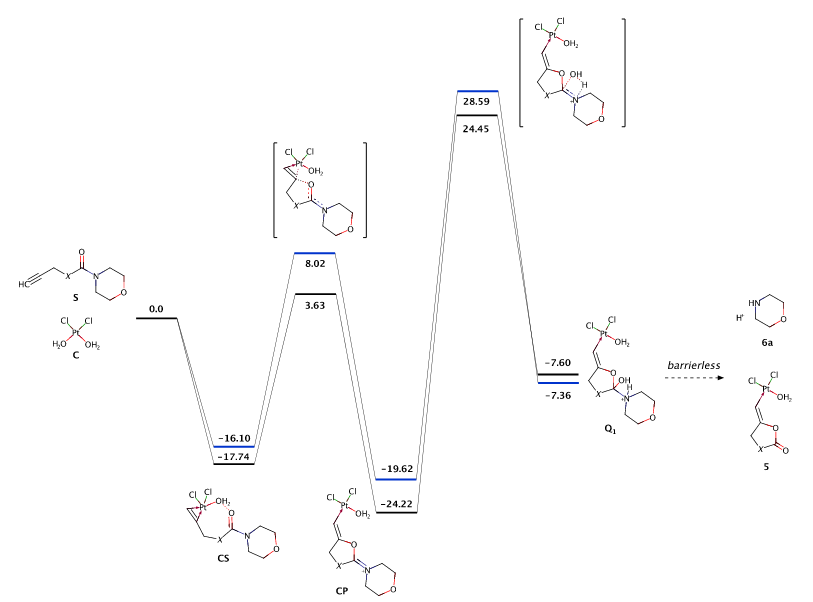
\includegraphics[width=0.95\textwidth]{slides/public/paper2-reaction}
	\caption{Summarized diagram of the proposed reaction mechanism in~\citeauthor{Oliveira_2020}.
		Energies are in~\kcalmol.
		Licensed under a
		Creative~Commons~CC-BY~license~\ccby~\cite{ACS_CCBY_2014}.}\label{fig:paper2-reaction}
\end{figure}

We discussed a new reaction of alkynes with platinum complexes that can be used to release secondary amines from tertiary amides,
which can be used to activate prodrugs.
This reaction was shown to occur through a platinum-mediated intramolecular cyclization mechanism,
and water was found to be a necessary metal-activating agent.
The reaction was also tested in mammalian cells and a colorectal cancer zebrafish xenograft model
and it was found to be successful in both cases.
The reaction was also adapted to work with~\ce{N}-propargyl groups and was used to synthesize a noninternalizing ADC.\@
To conclude,
our work revealed the suitability of platinum complexes for prodrug activation in physiological conditions,
demonstrating the potential of platinum-mediated decaging reactions
and paving the way for future developments and~\emph{in vivo} applications.

\section{Full text}

This work was a collaboration between researchers
at the Department of Chemistry at the Univerity of Cambridge,
the Molecular Medicine Institute at the University of Lissabon,
the Champalimaud Center for the Unknown at the Champalimaud Foundation,
the Department of Chemistry at the Federal University of Santa Catarina (UFSC),
and the FT-ICR and Structural Mass Spectroscopy Laboratory at the University of Lissabon.

The work was partially funded by the Brazilian Council for Scientific and Tecnological Development (CNPq),
grant/award numbers 140485/2017--1 and 311963/2017--0,
Coordination for the Improvement of Higher Education Personnel (CAPES),~PRINT programme call number 88887.310560--00.
See the acknowledgements session in the full print
(available at the end of this chapter)
for the complete list of international finantial aids.

The publication can be read in full next.
Given that this work was featured in the journal's cover,
it has received some local media coverage as well~\cite{noticias-da-ufsc2020}.~\citeauthor{Oliveira_2020}~\cite{Oliveira_2020}
is licensed under a
Creative~Commons~CC-BY~license~\ccby~\cite{ACS_CCBY_2014}.
A video showing the initial metadynamics simulation for the reaction is available at YouTube~\footnote{\url{https://youtu.be/k5ptn50Zjkc}}.

\includepdf[pages=-]{pubs/oliveira2020-paper2.pdf}
